\documentclass[12pt]{article}

\usepackage{answers}
\usepackage{setspace}
\usepackage{graphicx}
\usepackage{enumitem}
\usepackage{multicol}
\usepackage{mathrsfs}
\usepackage[margin=1in]{geometry} 
\usepackage{amsmath,amsthm,amssymb,mathtools}
\usepackage{titlesec}

\newcommand\numberthis{\addtocounter{equation}{1}\tag{\theequation}}

\titleformat{\section}[runin]{\normalfont\Large\bfseries}{\thesection}{1em}{}
\titleformat{\subsection}[runin]{\normalfont\large\bfseries}{\thesubsection}{1em}{}

\def\tf{\textbf}
\def\tt{\textit}
\def\mc{\ensuremath\mathcal}
\def\mf{\ensuremath\mathbf}
\def\mt{\ensuremath\mathit}
\def\mb{\ensuremath\mathbb}
\def\td{\ensuremath\tilde}
\def\N{\ensuremath\mb{N}}
\def\Z{\ensuremath\mb{Z}}
\def\C{\ensuremath\mb{C}}
\def\R{\ensuremath\mb{R}}
\def\S{\ensuremath\mb{S}}
\def\Ber{\ensuremath\mf{Ber}}
\def\det{\ensuremath\mf{det}}
\def\sigm{\ensuremath\mf{sigm}}
\def\diag{\ensuremath\mf{diag}}
\def\dom{\ensuremath\mf{dom}}
\def\cond{\ensuremath\mf{cond}}
\def\sign{\ensuremath\mf{sign}}
\def\bd{\ensuremath\mf{bd}}
\def\rto{\ensuremath\rightarrow\ }
\def\Rto{\ensuremath\Rightarrow\ }
\def\lto{\ensuremath\leftarrow\ }
\def\Lto{\ensuremath\Leftarrow\ }
\def\xrto{\ensuremath\xrightarrow}
\def\xRto{\ensuremath\xRightarrow}
\def\xlto{\ensuremath\xleftarrow}
\def\xLto{\ensuremath\xLeftarrow}
\def\rvec{\ensuremath\overrightarrow}
\def\lvec{\ensuremath\overleftarrow}

\providecommand\P[1]{}
\renewcommand\P[1]{\mb{P}\{#1\}}
\providecommand\E[1]{}
\renewcommand\E[1]{\mb{E}[#1]}
\providecommand\Var[1]{}
\renewcommand\Var[1]{\mf{Var}(#1)}
\providecommand\p[2]{}
\renewcommand\p[2]{\frac{\partial #1}{\partial #2}}
\providecommand\pp[2]{}
\renewcommand\pp[2]{\frac{\partial^2 #1}{\partial #2^2}}
\providecommand\ps[3]{}
\renewcommand\ps[3]{\frac{\partial^2 #1}{\partial #2\partial #3}}
\providecommand\d[2]{}
\renewcommand\d[2]{\frac{d #1}{d #2}}

\DeclareMathOperator{\sech}{sech}
\DeclareMathOperator{\csch}{csch}
    
\begin{document}
    
\title{Winding Numbers and Topology - Notes}
\author{Dhruv Kohli}
\maketitle
\section{Winding Number}
\begin{itemize}
    \item Winding number $\nu(L,p)$ of a closed loop $L$ about point $p$ is the net number of revolutions of the direction of $z$ as it traces out $L$ once in its given sense.
    \item A naive way to compute $\nu(L,p)$ is to start with a random point on $L$ and trace $L$ with your finger - starting with $0$, add $1$ for each positive (anti-clockwise) rotation of the arrow from $p$ to your finger and subtract $1$ for each negative (clockwise) rotation of the arrow from $p$ to your finger. When you have reached the starting point, the final count is the required winding number of the loop $L$ about $p$.
    \item A simple loop - one which does not intersect itself - divides plan into two just two sets, inside and outside (Proof is not easy). For a non-simple loop, this is not the case.
    \item A general loop $L$ divides the plane into a number of sets $D_{j}$. $\nu(L,p)$ is same for all $p$ in the same set. Proof: Consider a small segment of $L$. As $z$ traverses it, the rotation of $z-p$ will depend continuously on $p$ unless $p$ crosses $L$ i.e. if we move $p$ by a small amount then the rotation angle about the new point will differ from the original rotation by a small amount. Since winding number of loop about $p$ is nothing but the sum of rotations about $p$ due to all of its segments, it turns out that a small change in $p$ to $\td{p}$ will lead to small change in $[\nu(L,p)-\nu(L,\td{p})]$. But this must be an integer, so, it must be $0$.
    \item By above argument, we can assign a winding number $\nu_j$ to each set $D_j$. The "\tt{inside}" can now be defined as those sets with $\nu_j \neq 0$.
    \begin{figure}[h!]
        \centering
        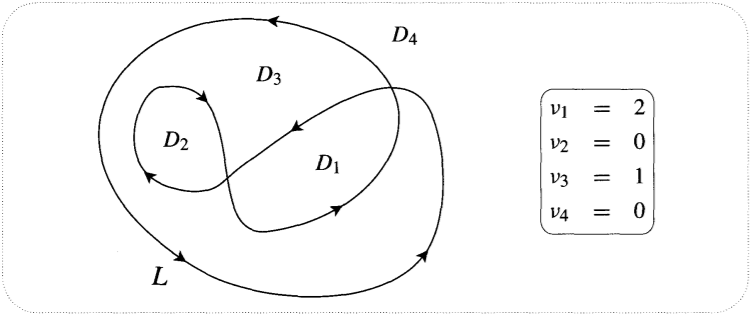
\includegraphics[scale=0.7]{fig_1}
        \label{f1}
    \end{figure}
    \item A quick way to compute winding numbers, 
    \begin{align*}
        &\tt{Crossing rule: If $L$ is moving from our left to our right (our right to our left)}\\
        &\tt{as we cross it, its winding number around us increases (or decreases) by one.} \numberthis \label{e1}
    \end{align*}

    \begin{figure}[h!]
        \centering
        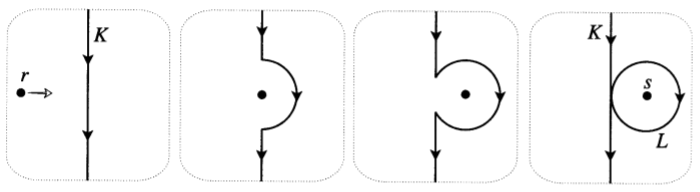
\includegraphics[scale=0.7]{fig_8}
        \label{f8}
    \end{figure}

    \item As a consequence of crossing rule, a ray emanating from a point $p$ such that it does not pass through self intersection point of loop and it is not tangent to loop, intersects the loop $|n| + 2m$ times where $m \in \N$.
\end{itemize}
\section{Hopf's Degree Theorem}
\begin{itemize}
    \item For a fixed loop and a continuously moving point, the winding number changes only when the point crosses the loop. The same is true for a fixed point and continuously moving loop. The winding number changes by $\pm 1$ if the continuously moving loop crosses the point. Thus if a loop $L$ can be continuously deformed into another loop $K$ without crossing point $p$ then $\nu(L,p) = \nu(K,p)$. It turns out that the converse is also true. 
    \begin{align*}
        &\tt{A loop $K$ may be continuously deformed to another loop $L$, without}\\
        &\tt{ever crossing the point $p$, if and only if $K$ and $L$ have the same}\\
        &\tt{winding number round $p$.} \numberthis \label{e2}
    \end{align*}
    \item Note that in three dimensions, a sphere encloses points inside it just once, like a circle in two dimensions enclosing points inside it just once. Hopf's theorem says that one closed surface may be continuously deformed into another closed surface, without ever crossing $p$, if and only if they enclose $p$ the same number of times. Indeed, the same is true for $n$-dimensional surfaces in $(n+1)$-dimensional space.
    \item Proof of converse of Hopf's theorem in $2$ dimensions is as follows - 
    \begin{itemize}
        \item Consider a unit circular rubber band $C$ around origin which is continuously deformed into an arbitrary loop $L$ around origin (i.e. rubber band may cross the origin while deforming).
        \begin{figure}[h!]
            \centering
            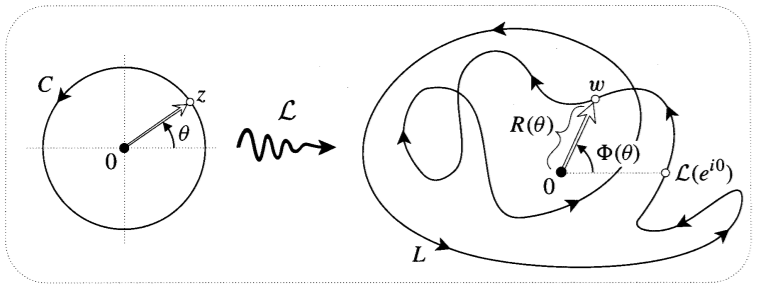
\includegraphics[scale=0.7]{fig_2}
            \label{f2}
        \end{figure}
        \item The new loop $L$ can be represented as a mapping from the unit circle $C$ to $L$ given by $w = \mc{L}(z) = \mc{L}(e^{i\theta}) = R(\theta)e^{i\Phi(\theta)}$ where $R$ and $\Phi$ are continuous functions of $\theta$, so that $\mc{L}(C)=L$.
        \item We can always rotate $L$ so that $\mc{L}(0) = 0$. As $\theta$ goes from $0$ to $2\pi$, $z$ goes around $C$ once and $w$ goes around $L$ once. The net rotation of $w$ after it has returned to its initial point is given by $\Phi(2\pi) = 2\pi\nu$.
        \item To remove the distraction of the varying length $w$, we pull each point $w$ radially onto $w/|w|$ on the unit circle obtaining a standardized version of $L$ i.e. $\hat{L}$. The deformation from $L$ to $\hat{L}$ can be represented as $\mc{L}_{s}(z) = w + s(\hat{w}-w)$ where $s \in [0,1]$. As $s$ varies from $0$ to $1$, $\mc{L}_{s}(C)$ changes from $L$ to $\hat{L}$.
        \item Note that in this process origin is never crossed.
        \begin{figure}[h!]
            \centering
            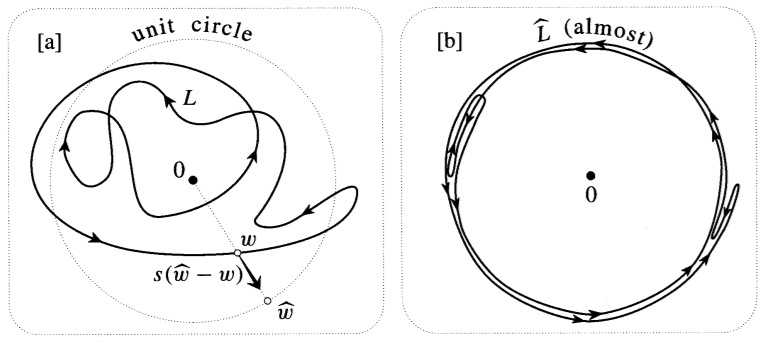
\includegraphics[scale=0.7]{fig_3}
            \label{f3}
        \end{figure}
        \item So, $\hat{w} = \hat{\mc{L}}(e^{i\theta}) = e^{i\Phi(\theta)}$. Note that $\Phi(\theta)$ completely describes this mapping. As $z$ moves around $C$ with unit speed, $\hat{w}$ moves around $\hat{L}$ with speed $|\Phi'(\theta)|$ at $\theta$.
        \item The archetypal mapping of degree $\nu$ is given by $\hat{\mc{J}_{\nu}}(z)=z^{\nu}$, for which $\Phi(\theta)=\nu\theta$. As $z$ goes around $C$ with unit speed, $\hat{w}$ travels around $\hat{J_{\nu}}$ with constant speed $|\nu|$, completing $|\nu|$ circuits of unit circle.
        \item Recall that $C$ was made of a rubber band. Thinking of unit circle as boundary of a solid cylinder, as $\hat{L}$ is released, it contracts to $\hat{J_{\nu}}$. This process of taking up slack can be described in terms of the graph of $\Phi$ i.e. $\Phi_{t}(\theta) = \Phi(\theta)+t(\nu\theta - \Phi(\theta)$ where as $t$ varies from $0$ to $1$, $\Phi_{t}$ from original $\Phi$ to straight line graph of archetype.
        \begin{figure}[h!]
            \centering
            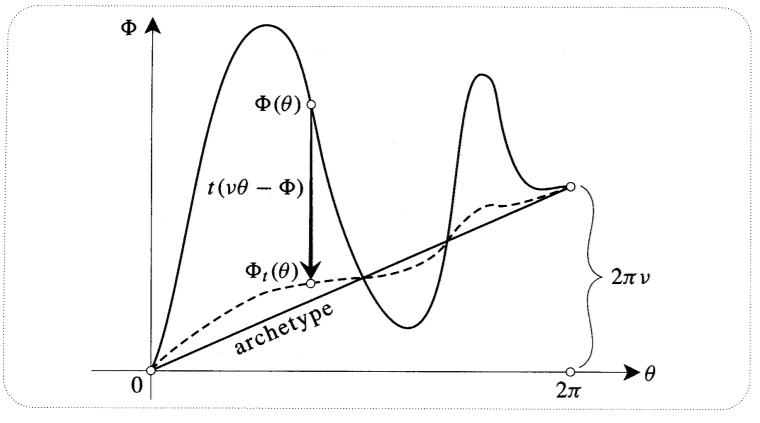
\includegraphics[scale=0.7]{fig_4}
            \label{f4}
        \end{figure} 
        \begin{align*}
            &\tt{Any $\hat{L}$ of winding number $\nu$ can be continuously deformed}\\
            &\tt{to archetypal loop $\hat{J_{\nu}}$ and vice versa.} \numberthis \label{e3}
        \end{align*}
        \item Defining $\hat{\mc{L}_{t}}(e^{i\theta}) = e^{i\Phi_{t}(\theta)}$, $\hat{\mc{L}_{t}}(C)$ evolves continuously and reversibly from $\hat{L}$ to $\hat{J_{\nu}}$ as $t$ varies from $0$ to $1$.
        \item Finally, if $K$ and $L$ have same winding number $\nu$ then $K$ can be deformed to $\hat{J_{\nu}}$ which can further be deformed to $L$ by reversing the steps of deformation of $L$ to $\hat{J_{\nu}}$.
    \end{itemize}
\end{itemize}
\section{Polynomials and the Argument Principle}
\begin{align*}
    &\tt{If $f(z)$ is analytic on and inside $\Gamma$, and $N$ is the number}\\
    &\tt{of $p$-points [counted with their multiplicities] inside}\\
    &\tt{$\Gamma$, then $N=\nu[f(\Gamma),p]$.} \numberthis \label{e4}
\end{align*}
\begin{figure}[h!]
    \centering
    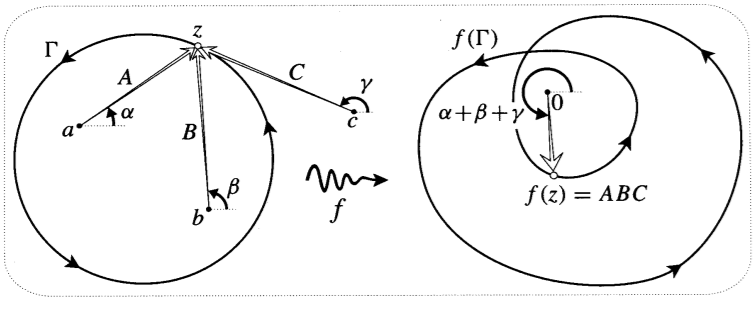
\includegraphics[scale=0.7]{fig_5}
    \label{f5}
\end{figure}
\section{A Topological Argument Principle}
\subsection{Counting Preimages Algebraically}
\begin{align*}
    &\tt{For an analytic function $f(z)$ s.t. $f(a)=p$ that is $a$ is a preimage}\\
    &\tt{of $p$, algebraic multiplicity (order or valence) of $a$ is defined as}\\
    &\tt{the degree of the dominant term in the Taylor series expansion of}\\
    &\tt{$f(z)-p$ about $a$.} \numberthis \label{e5}
\end{align*}
\begin{align*}
    f(z)-p = f(z)-f(a) = \frac{f'(a)}{1!}(z-a) + \frac{f''(a)}{2!}(z-a)^2 + \ldots \numberthis \label{e6}
\end{align*}
\begin{itemize} 
    \item If $f'(a)\neq 0$ then algebraic multiplicity of $a$ is $1$ and $a$ is called \tt{simple} root of $f(z)-p$.
    \item The first nonzero term on right is one that dominates the local behaviour of $f(z)-p$.
    \item Note that the above definition solely depends on the fact that analytic functions can always be represented as a convergent Taylor series.
    \item Also, note that when the algebraic multiplicity of $a$ is $n$ s.t. $n>1$ i.e. the dominanting term in the Taylor series of $f(z)-p$ is $f^{(n)}(z-a)^{n}/n!$, then $f^{(n)}(a)$ is the first nonvanishing derivative of $f$ at $a$ and, therefore, $a$ is also a critical point of $f$ of order $n-1$.
    \item Little geometric intuition of above point - If $f'(a)\neq 0$ the an infinitesimal disc centered at $a$ is amplitwisted to an infinitesimal disc centered at $0$, so that points close to $a$ cannot map to $0$.
    \begin{figure}[h!]
        \centering
        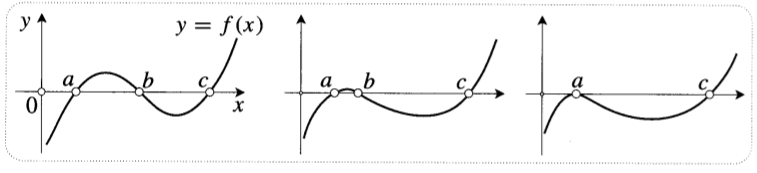
\includegraphics[scale=0.7]{fig_6}
        \label{f6}
    \end{figure}
    \item If root $a$ of polynomial $P(z)$ has multiplicity $n$ then $P$ may be factorizaed as $(z-a)^n\Omega(z)$, where $\Omega(a)\neq 0$.
    \item If $a$ is a $p$-point of $f$ of algebraic multiplicity $n$ then, by equation \eqref{e6} we have, $f(z)-p = \Omega(z)(z-a)^n$ where $\Omega(z) = \frac{f^{(n)}(a)}{n!} + \frac{f^{(n+1)}(a)}{(n+1)!}(z-a) + \ldots$.
    \item Note that from this point of view, the only difference between analytic mapping and a polynomial is that the latter has a single "once and for all" factorization while the former requires different factorization in the neighbourhood of each $p$-point.
\end{itemize}
\subsection{Counting Preimages Geometrically}
\begin{itemize}
    \item We can further generalize \eqref{e4} for mappings that are just continuous. The very notion of algebraic multiplicity is meaningless for such general mappings (because Taylor series expansion may not converge). So, we need a geometric way of counting preimages that will agree with the previous defintion of algebraic multiplicity \eqref{e5} if we specialize to analytic mappings.
    \item Condider an analytic mapping $f$ with $p$-point $a$. Consider an infinitesimal circle $C_a$ centred at $a$. If $a$ is simple i.e. $f'(a)\neq 0$ then $C_a$ is amplitwisted to an infinitesimal circle at $p$. The winding number of this image circle around $p$ is $1$ which is same as the algebraic multiplicity of $a$.
    \item Now, suppose algebraic multiplicity of $a$ is $n$. Then, $f(z) = p + \Omega(z)(z-a)^{n}$ with $\Omega(a)\neq 0$. Thus, as $z$ revolves around $a$ once, $z-a$ revolves $0$ once and $(z-a)^n$ revolves around $0$ $n$ times. As $C_a$ is made smaller approaching to point $a$, $\Omega(C_a)$ approaches to $\Omega(a)\neq 0$. Therefore, we can choose $C_a$ small enough so that winding number of $\Omega(C_a)$ about $0$ is $0$. Finally we have,
    \begin{align*}
        \nu[f(C_a),p] = \nu[f(C_a)-p,0] = \nu[(C_a-a)^n\Omega(C_a),0] = \nu[z^n,0] + \nu[\Omega(C_a),0]=n \numberthis \label{e7}
    \end{align*}
    \item Now to define multiplicity of a mapping $h(z)$ that is merely continuous - Let $\Gamma_a$ be any simple loop round $a$ that does not contain other $p$-points. If we continuously deform $\Gamma_a$ to $\td{\Gamma}_a$ with crossing $a$ or any other $p$-point then $h(\Gamma_a)$ will continuously deform into $h(\td{\Gamma}_a)$ without ever crossing $p$, and so $\nu[h(\td{\Gamma}_a),p] = \nu[h(\Gamma_a),p]$.
    \item Thus, without specifying $\Gamma_a$ further, we may define topological multiplicity (local degree of $h$ at $a$) of $a$ to be $\nu(a) = \nu[h(\Gamma_a),p]$.
    \item By deforming $\Gamma_a$ into infinitesimal circle $C_a$ for an analytic mapping one can note that the two types of multiplicites agree with each other.
\end{itemize}
\subsection{What's Topologically Special About Analytic Functions?}
\begin{itemize}
    \item 
    \begin{align*}
        &\tt{$\nu(a)$ is always positive for analytic functions,}\\
        &\tt{while it can be negative for nonanalytic functions.} \numberthis \label{e8}
    \end{align*}
    \item For example, $h(z)=\bar{z}$ has topologically multiplicity of $-1$ everywhere.
    \item Recall that local effect of a nonanalytic mapping that is differentiable in the real sense (i.e. $u(x,y)$ and $v(x,y)$ are differentiable functions of $x$ and $y$) at a $p$-point $a$ consist of (after translation to $p$) a stretch by some factor $\xi_a$ in one direction, another stretch by some factor $\eta_a$ in perpendicular direction and a rotation through some angle $\phi_a$. For such a mapping, an infinitesimal circle $C_a$ centred at $a$ will distort into an infinitesimal ellipse $E_p$ centred at $p$. If both expansion factors have same sign then the mapping preserves orientation so that $E_p$ circulates in the same sense as $C_a$ and $\nu(a) = +1$ otherwise orientation is reversed and $\nu(a)=-1$. Note that $\xi_a$ and $\eta_a$ are NOT the eigenvalues of $J(a)$. Also, note that $\det J(a)$ measure the local expansion factor of the area at $a$ (including sign for the orientation). In summary,
    \begin{align*}
        \nu(a) &= \text{the sign of } (\xi_a\eta_a)\\ 
        &= \text{the sign of } \det[J(a)]\\
        &= \text{the sign of } (\lambda_1(a)\lambda_2(a)) \numberthis \label{e9}
    \end{align*}
    \item If $\det[J(a)]=0$ then the formula cannot be used. The behaviour of the mapping is locally crushing at $a$. As for analytic mappings, such a place is called a critical point.
    \item But, local crushing at a critical point of an analytic mapping is perfectly symmetrical in all directions (both expansion factors/eigenvalues are equal), this may not be the case for the nonanalytic mappings that are differentiable in the real sense. For example, if $f(x+iy)=x-iy^3$ then $\det[J]=-3y^2$ clearly horizontal separation of points are left as it is, but all points on the real axis are critical points as a result of crushing in the vertical direction.
    \begin{align*}
        &\tt{The critical points of an analytic mapping can be distinguished}\\
        &\tt{purely on the basis of topological multiplicity; those}\\
        &\tt{of a nonanalytic mapping cannot.} \numberthis \label{e10}
    \end{align*}
    \item For analytic functions $\nu(a)=+1$ iff $a$ is not critical. In the nonanalytic case $\nu(a)=\pm 1$ if $a$ is not critical, but it is also possible for a critical point to have these multiplicities. As in the example above the points on the real axis are critical but have topological multiplicity of $-1$.
    \begin{align*}
        &\tt{$\nu(a)$ is never zero for analytic mappings, but it can}\\
        &\tt{vanish for non-analytic mappings.}\numberthis \label{e11}
    \end{align*}
    \item For example, points on real axis of $f(x,y)=x+i|y|$ have multiplicity of $0$.
\end{itemize}
\subsection{A Topological Argument Principle}
\begin{itemize}
    \item Let $\Gamma$ be a simple loop, and let $h(z)$ be a continuous mapping such that only a finite number of its $p$-points lie inside $\Gamma$.
    \begin{align*}
        &\tt{The total number of $p$-points inside $\Gamma$ (counted }\\
        &\tt{with their topological multiplicities) is equal to the winding}\\
        &\tt{number of $h(\Gamma)$ around $p$.} \numberthis \label{e12}
    \end{align*}
    \item Proof:
    \begin{figure}[h!]
        \centering
        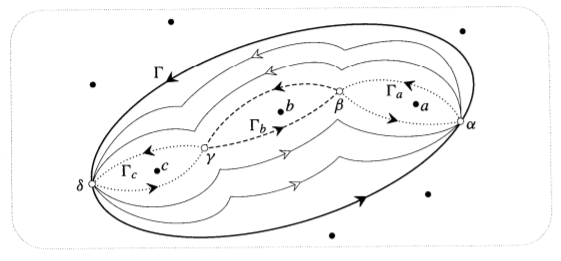
\includegraphics[scale=0.7]{fig_7}
        \label{f7}
    \end{figure}
    \begin{itemize}
        \item Consider three $p$-points $a$, $b$ and $c$ lying inside $\Gamma$ while others lie scattered outside.
        \item $\Gamma$ can be deformed into doubly pinched loop $\alpha\beta\gamma\delta\gamma\beta\alpha$ which we call $\td{\Gamma}$.
        \item Since no $p$-points were crossed $h(\Gamma)$ will wind round $p$ same number of times as $h(\td{\Gamma})$.
        \item $\td{\Gamma}$ is made up of $\Gamma_a=\alpha\beta\alpha$, $\Gamma_b=\beta\gamma\beta$, $\Gamma_c = \gamma\delta\gamma$.
        \item winding numbers of their images round $p$ are, by definition, topological multiplicities of $a$, $b$ and $c$.
        \item Let $\mc{R}(K)$ be the net rotation of $h(z)$ round $p$ as $z$ traverses $K$. If $K$ is closed then $\mc{R}(K) = 2\pi \nu [h(K),p]$. Then,
        \begin{align*}
            2\pi \nu[h(\Gamma),p] &= 2\pi \nu[h(\td{\Gamma}), p]\\
            &= \mc{R}(\alpha\beta\gamma\delta\gamma\beta\alpha)\\
            &= \mc{R}(\alpha\beta) + \mc{R}(\beta\gamma) + \mc{R}(\gamma\delta) + \mc{R}(\delta\gamma) + \mc{R}(\gamma\beta) + \mc{R}(\beta\alpha)\\
            &= \mc{R}(\alpha\beta\alpha) + \mc{R}(\beta\gamma\beta) + \mc{R}(\gamma\delta\gamma)\\
            &= \mc{R}(\Gamma_a) + \mc{R}(\Gamma_b) + \mc{R}(\Gamma_c)\\
            &= 2\pi[\nu(a) + \nu(b) + \nu(c)]
        \end{align*}
        \item This extends to any number of $p$-points $a_1$, $a_2$ etc. lying inside $\Gamma$:
        \begin{align*}
            \nu[h(\Gamma),p] = \sum\limits_{\text{inside }\Gamma} \nu(a_j)
        \end{align*}
    \end{itemize}
    \item A consequence of above principle is \tt{Darboux's Theorem}:
    \begin{align*}
        &\tt{Let $\Gamma$ be a simple loop. If an analytic function $h$ maps $\Gamma$ onto $h(\Gamma)$}\\
        &\tt{in one-to-one fashion, then it also maps the interior of $\Gamma$}\\
        &\tt{onto the interior of $h(\Gamma)$ in one-to-one fashion.}
    \end{align*}
    Firstly, since $\Gamma$ is a simple loop and $\Gamma \rto h(\Gamma)$ is a one to one map i.e. $h(x_1)=h(x_2)\implies x_1 = x_2$ for all $x_1,x_2\in \Gamma$, we have $h(\Gamma)$ is also a simple loop. Now, if $p$ inside $h(\Gamma)$ has more than one preimage then it must have a winding number of more than $1$ which is a contradiction (because $h(\Gamma)$ is a simple loop $p$ has winding number of $1$). So, $p$ must have exactly one preimage inside $\Gamma$. Done.
\end{itemize}
\section{Rouche's Theorem}
\subsection{The Result}
\begin{itemize}
    \item Let $\Gamma$ be a simple loop. If $|g(z)|<|f(z)|$ on $\Gamma$, then $\nu[(f+g)(\Gamma),0] = \nu[f(\Gamma),0]$. This can be seen by the analogy of tree-man-dog-walk.
    \item By the Argument Principle, we have, \tt{Rouche's Theorem}.
    \begin{align*}
        &\tt{If $|g(z)|<|f(z)|$ on $\Gamma$, then $(f+g)$ must have the}\\
        &\tt{same number of zeros inside $\Gamma$ as $f$.}
    \end{align*}
    $|g(z)| < |f(z)|$ is a sufficient, not a necessary condition for $(f+g)$ to have same number of roots as $f$. Example, $g(z)=2f(z)$ has same number of roots but $|g(z)| = 2|f(z)| \geq |f(z)|$.
\end{itemize}

\subsection{The Fundamental Theorem of Algebra}
\begin{itemize}   
    \item Using Rouche's theorem one can prove the fundamental theorem of algebra, which states that a polynomial

    \begin{align*}
        P(z) &= z^n + Az^{n-1} + Bz^{n-2} + \ldots +E
    \end{align*}

    of degree $n$ always has $n$ roots.
    \item Proof: let $f(z) = z^n$ and $g(z) = Az^{n-1} + Bz^{n-2} +\ldots + E$. Let $C$ be the circle $|z| = 1+|A| + |B| + \ldots + |E|$. Since $|z|>1$ on $C$,
    
    \begin{align*}
        |g(z)| &= |Az^{n-1}+Bz^{n-2}+\ldots+E|\\
        &\leq |A||z^{n-1}| + |B||z^{n-2}| + \ldots |E|\\
        &< |A||z|^{n-1} + |B||z|^{n-1} + \ldots + |E||z|^{n-1}\\
        &= |f(z)|
    \end{align*}

    Using Rouche's theorem we have the number of preimages of $f(z)$ in $C$ (which is $n$) is equal to the number of preimages of $f(z)+g(z)=P(z)$ in $C$.
\end{itemize}

\subsection{Brouwer's Fixed Point Theorem}
\begin{itemize}
    \item \tt{Any continuous mapping of the disc to itself will have a fixed point}. Physical analogy: Talcum powder on coffee.
    \item Showing that there must be a fixed point if the disc is mapped into its interior and there are at most a finite number of fixed points.
    \begin{itemize}
        \item Let $D$ be $|z|\leq 1$. Let $g$ map $D$ to its interior i.e. $|g(z)|<1$ for all $z \in D$. Let $m(z)$ be the movement of $z$ under $g$ i.e. $m(z)=g(z)-z$. A fixed point corresponds to no movement. Let $f(z) = -z$. Then, on the boundary of $D$, $|g(z)| < 1 = |f(z)|$. So, $m(z)=g(z)+f(z)$ has same number of roots inside $D$ as $f$ i.e. one.
        \item If $g$ is merely continuous then there can be several fixed points, some of which will necessarily have negative multiplicities, while if $g$ is analytic then there can literally be one fixed point.
    \end{itemize}
\end{itemize}
\section{Maxima and Minima}
\subsection{Maximum-Modulus Theorem}
\begin{itemize}
    \item \tt{If $f$ is analytic inside and on a simple loop $\Gamma$ then no point outside $f(\Gamma)$ can have a preimage inside $\Gamma$}. Proof: $\sum_{\text{preimages } a_{j} \text{ inside } \gamma}\nu(a_j) = 0$. Since, $\nu(a_j)>0$ for analytic mapping, therefore, no preimage inside $\gamma$.
    \item If $p$ lies inside $f(\Gamma)$ then $\nu[f(\Gamma),p]\neq 0$ and so there must be atleast one preimage inside $\Gamma$. This is true for nonanalytic mappings too.
    \item \tt{The maximum of $|f(z)|$ on a region where $f$ is analytic is always achieved by points on the boundary, never ones inside}. This is called \tt{Maximum-Modulus Theorem}. Only exception is the trivial analytic mapping $z\rto \text{const}$. So, if an analytic $f$ achieves maximum at an interior point then $f$ must be constant.
    \item The modular surface of analytic $f$ does not even have a local maximum on an interior point, because if it does then for a small loop about that point, the highest point will fail to lie on the boundary of the loop. Another way to see this is by drawing a small loop $\gamma$ about $p$ and the image loop $f(\gamma)$. Since there are points away from $f(p)$ in all directions, a ray emanating from origin pointing directly away from origin, will meet the $f(\gamma)$ at some point which will correspond to the point with maximum modulus.
    \item \tt{For analytic function, unless there is a $0$-point inside $\Gamma$, at which $|f(z)|=0$, the points $Q$ closest to origin (minimum $|f(z)|$) must also be the image of a point $q$ lying on the boundary $\Gamma$}. This is called \tt{Minimum-Modulus Theorem}. Thus, there can be no pits in the modulur surface of analytic function, unless the surface actually hits the complex plane at an interior $0$-point of $f$.
    \item Only exception is the constant function. So, if an analytic $f$ achieves minimum (positive) modulus at an interior point then $f$ must be constant.
\end{itemize}
\section{Schwarz-Pick Lemma}
\section{The Generalized Argument Principle}
\subsection{Rational Functions}
\begin{itemize}
    \item \tt{Let $f$ be analytic on a simple loop $\Gamma$ and analytic inside except for a finite number of poles. If $N$ and $M$ are the number of $p$-points and poles, both counted with their multiplicities, then $\nu[f(\Gamma),p]=N-M$}.
    \item Figure shows how it works in case of the mapping $f(z)=((z-a)(z-b))/(z-c)$. As such $f(z)$ goes to $\infty$ as $z\rto c$ but after that it comes back from $\infty$ and unwinds.
    \begin{figure}[h!]
        \centering
        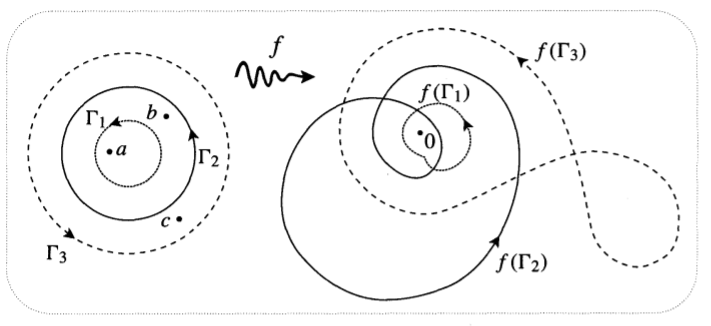
\includegraphics[scale=0.7]{fig_9}
        \label{f9}
    \end{figure}
    \begin{figure}[h!]
        \centering
        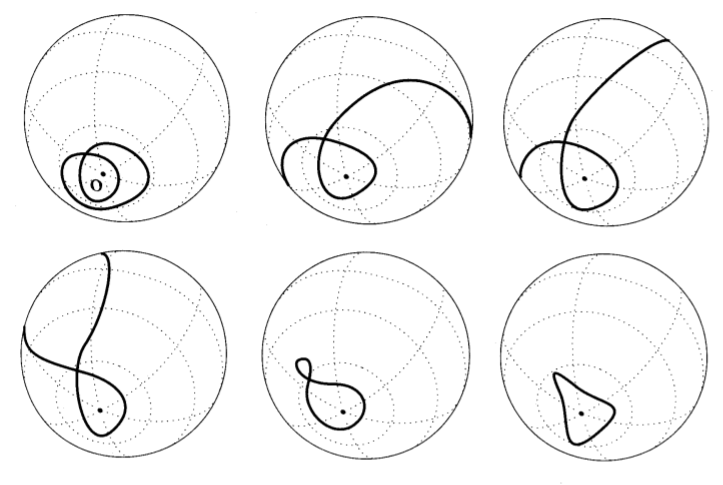
\includegraphics[scale=0.7]{fig_10}
        \label{f10}
    \end{figure}
\end{itemize}
\subsection{Poles and Essential Singularities}
\begin{itemize}
    \item Two kinds of singularities exist for an otherwise analytic function:
    \begin{enumerate}
        \item Pole: It is the type to which (17) applies to. If $f(z)$ approaches infinity as $z$ approaches $a$ from any directions then $a$ is a pole of $f$. In the modular surface, there will be an infinitely high spike, a ``pole'' at $a$. Since $f$ is analytic $F=1/f$ is also analytic and has a root at $a$. If this root has multiplicity $m$ then $F(z)=(z-a)^m\Omega(z)$ where $\Omega(a)\neq 0$. The local behaviour of $f$ near $a$ is thus, $f(z)=\td{\Omega}(z)/(z-a)^m$ where $\td{\Omega}(z)=1/\Omega(z)$ is analytic and nonzero at $a$. $m$ is defined as the algebraic multiplicity or order of the pole. This is the order of first nonvanishing derivative of $1/f$. The function $f$ is called meromorphic in a region if the only singularities present in the region are poles.
        \item Essential Singularities: If analytic $f$ has an essential singularity at $f$ then it must be unbounded in the vicinity of $s$ (otherwise it will not be a singularity) and $f$ must not approach to infinity from all directions as $z\rto s$ (otherwise it will be a pole). Example $g(z)=e^{1/z}$. $|g(z)|=e^{\cos\theta}/r$. If $z\rto 0$ along imaginary axis $|g(z)|=1$. But if the approach is along a path on the left of imaginary axis then $|g(z)|\rto\infty$. \tt{The rate at which is zooms off to $\infty$ is beyond the ken of any pole}.
    \end{enumerate}
\end{itemize}
\subsection{The Explanation}
\begin{itemize}
    \item If $f(z)=\Omega(z)(z-a)^m$ where $\Omega(a)\neq 0$ then as $z$ traces a small circle around $a$, $f$ will wind around origin $m$ times. Projecting on Riemann sphere, we get a loop winding around south pole $m$ times. Now if we apply complex inversion to $f$ to get $F(z)=\td{\Omega}(z)/(z-a)^m$, on Riemann sphere, since complex inversion results in rotation of $\pi$ about real axis, the loop winding south pole will now wind north pole $m$ times in counterclockwise sense as seen from inside the sphere. The stereographic projection of this loop will be a a large loop winding around $0$, $m$ times in clockwise sense.
    \item \tt{If $a$ is a pole of order $m$ and $\Gamma_a$ is any simple loop containing $a$ but no $p$-points and no other poles, then $\nu[f(\Gamma_a),p] = -m$}.
    \begin{align*}
        \nu[f(\Gamma),p] &= \sum_{p\text{-points}}\nu[f(\Gamma_{a_j}),p] + \sum_{\text{poles}}\nu[f(\Gamma_{s_j}),p]\\
        &= [\text{no. of $p$-points inside $\Gamma$}] - [\text{no. of poles inside $\Gamma$}]
    \end{align*}
\end{itemize}
\end{document}
    